\documentclass[sigplan,11pt,screen,nonacm]{acmart}
\settopmatter{printacmref=false}
\setcopyright{none}
\usepackage{hyperref}
\usepackage[ngerman]{babel}
% Titel "Zusammenfassung" zu "Abstract" ändern
\addto\captionsngerman{\renewcommand{\abstractname}{Abstract}}

\begin{document}
% Festlegung Art der Zitierung - Havardmethode: Abkuerzung Autor + Jahr
\bibliographystyle{alphadin}

% Sorgt für Silbentrennung und Einhaltung der Spaltenbreite
\sloppy

\interfootnotelinepenalty=10000
	
\title{Decentralized Web}
\subtitle{Das Internet der Zukunft?}

\author{Benedikt Weber}
\email{benedikt.weber@mni.thm.de}

%% A "teaser" image appears between the author and affiliation
%% information and the body of the document, and typically spans the
%% page.
\begin{teaserfigure}
	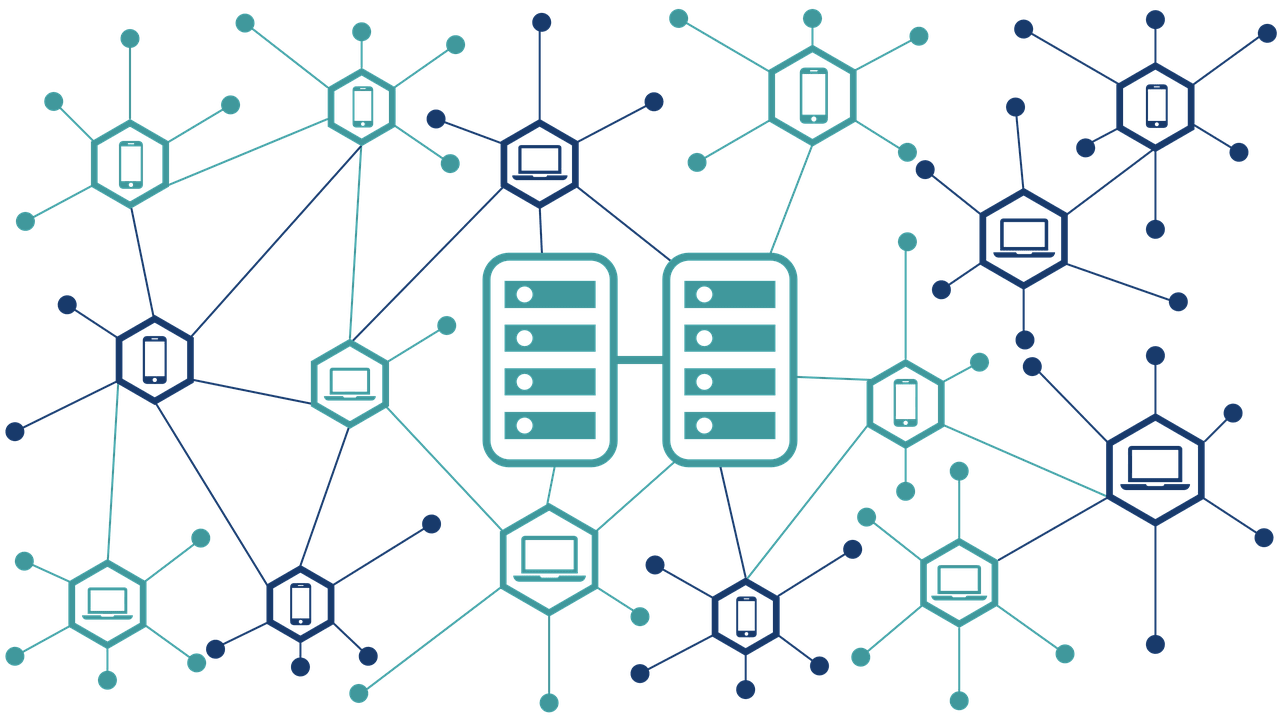
\includegraphics[width=\textwidth]{images/teaser}
	\caption{Beispielhaftes Konzept eines dezentralen Netzwerks~\cite{shivang.2018}}
	\label{fig:teaser}
	\bigskip
\end{teaserfigure}

%%
%% The abstract is a short summary of the work to be presented in the
%% article.
\begin{abstract}
	The following paper deals with the question if the technology of a decentralized web could possibly be used in the future while replacing the currently well-established client-server architecture.
	
	To discuss this question properly a wide range of knowledge over the current situation and the functionality of a decentralized web is necessary.
	
	The paper starts with the explanation, why the term Web3 is used over the counterpart Web 3.0, which is because Web 3.0 references more the concept of a semantic web, while Web3 is mostly used while talking about the use case of blockchain in a new era of the internet.
	
	It continues by giving insights on how the client-server architecture works and how the technology evolved over time to it's current state.
	
	Also the major problems this architecture involves are extensively described, because these are the main reasons why a development towards a decentralized web is strongly needed. This includes (1) huge privacy issues regarding tech giants like GAFA
	\footnote{
		\textbf{G}oogle, \textbf{A}pple, \textbf{F}acebook und \textbf{A}mazon
	}
	stockpiling customer data (2) the need of web services or platforms which act as intermediaries. Not only trusting them is a huge issue, these servers are more likely to be attacked which sometimes ends in downtimes or even data thefts.
	
	\smallskip
	
	These problems could be solved by peer-to-peer networks and the use of blockchain. This massively increasing technology enables clients to not only use web services but provide them to others simultaneously. In this case the omission of intermediate platforms holds huge advantages, amongst others (1) security improvements, because there is no such thing like one server that could be attacked (2) control over private data, because everyone is in the position to delete his data whenever he wants.
	
	The problem with this technology lies in the implementation, because bugs which are not located beforehand can end in huge problems.
	
	\smallskip
	
	Therefore it is still a long way to a decentralized web, but there are already many organizations and companies working on it to improve every single aspect, in order to fulfill a transition to a free and safe web as it was intended to by it's founder.	
	
\end{abstract}



\maketitle

\section{Einleitung}

Seitdem das Internet für die Öffentlichkeit freigegeben wurde, hat es sich in kurzer Zeit sehr
stark entwickelt. Zu Beginn wurden immer mehr Computer miteinander verbunden, was den
Datenaustausch massiv beschleunigte. Durch die Einführung der Standards von Tim Berners-Lee um 1990~\cite{Krause.2008} wurde es relativ einfach, Webseiten mit wenigen Zeilen Code
darzustellen. Dies ermöglichte es den Nutzern, schnell auf Informationen und Ressourcen
zuzugreifen, die Navigation erfolgte dabei im Web durch Hyperlinks und Suchmaschinen. Diese
Phase reicht bis ins Jahr 2003 und wird als Web~1.0 bezeichnet. Als Killer-Applikation
\footnote{
	\label{footnote:KillerAnwendung}Eine Anwendung, die einer bestimmten Technik zum Durchbruch verhalf~\cite{Duden.2019}
}
gilt der Web-Browser, der den Menschen Zugang zum World Wide Web gewährte. Mit der Einführung
von Social-Media- und e-Commerce-Plattformen brach die Phase des sogenannten Web~2.0 an,
in der wir uns derzeit befinden. Diese Phase wird als Frontend-Revolution bezeichnet~\cite[S. 23]{Voshmgir.2019}. Der bedeutendste Unterschied liegt dabei in der Zugriffsart: Während
das Web~1.0 den Nutzern überwiegend lesenden Zugriff auf Ressourcen bot, konnten die Nutzer
am Web~2.0 partizipieren und soziale Interaktionen durchführen. Im Web~1.0 gab es also Webseiten eines Betreibers, die sich Nutzer ansehen konnten. Im Web~2.0 standen dann Seiten wie Wikipedia zur Verfügung, deren Inhalt verschiedenste Seitenbesucher bearbeiten konnten. Für solchen Interaktionen wird jedoch immer ein Mittelsmann benötigt, also eine Plattform, die zwei Personen, die sich nicht kennen und nicht vertrauen, eine Möglichkeit des Austauschs bietet. Die dahinterliegende Infrastruktur nennt sich Client-Server-Architektur: Ein Server stellt einen Dienst zur Verfügung, auf den mehrere Clients Zugriff erhalten und sich somit untereinander verknüpfen können.

\smallskip

Doch obwohl es immer mehr Endgeräte mit Zugang zum Web gibt~\cite{CiscoSystems.2011}, hat sich diese Struktur nicht verändert. Das Problem an dieser Stelle: Es entstehen Abhängigkeiten von den einzelnen Servern, die mitt\-ler\-wei\-le eine Vielzahl von Clients bedienen müssen, und die einen SPoF
\footnote{
	Single Point of Failure: Die Komponente eines Systems, ohne die das System nicht betriebsbereit ist~\cite{ITWissen.info.2017}
}
darstellen. 
Und diese technischen Aspekte sind nicht einmal die größten Probleme, die das World Wide Web heute mit sich bringt. 
Denn Abhängigkeiten bestehen auch zwischen den Nutzern und den Anbietern der Web-Dienste, wodurch bei großen Nutzerzahlen enormer Einfluss auf die Gesellschaft ausgeübt werden kann. 
Des Weiteren verdrängen oft Tech-Giganten wie Google, Apple, Facebook oder Amazon~\cite{Beutelsbacher.2016} die Konkurrenz vom Markt, wodurch Nutz\-ern oft keine richtigen Optionen bei der Auswahl der Dienste bleibt, denen sie ihre Daten anvertrauen. 
Dabei haben laut einer Umfrage Ende 2017 in
Deutschland lediglich 32\% der Befragten Vertrauen bezüglich der Einhaltung des
Datenschutzes in Google, bei Facebook sind es gerade einmal 18\%~\cite{Horizont.2017}.
Kommuniziert ein Client mit einem Server, speichert dieser Informationen über den Client,
und der Nutzer gibt mit jedem Request einen Teil der Kontrolle über seine Privatsphäre preis~\cite[S. 21]{Voshmgir.2019}.

Aus dieser Kritik heraus entstand die Idee des Decentralized Web, auch Web3 genannt. Beim
Konzept der Dezentralisierung wird die Architektur von Clients und Servern aufgebrochen,
denn das Netzwerk wird von „alle[n] Nutzer[n] und ein[em] Netzwerk unabhängiger Rechner
und Server“~\cite{Bonset.2019} betrieben. Im Web3 verändert sich das Frontend, also die Seiten, wie sie heute existieren, nicht. Stattdessen verändert sich das Backend massiv, da andere grundlegende Technologien benötigt werden.

\smallskip

Das Ziel dieser Seminararbeit soll sein, dem Leser oder der Leserin einen einfachen und
verständlichen Einblick in das Thema der Dezentralisierung zu gewähren, da das Web seine
Geschichte des schnellen Wandels fortführen wird. Dabei stellt das Decentralized Web als
solches eine Möglichkeit der Weiterentwicklung des heutigen Internets dar. Des Weiteren ist
es wichtig, den Nutzern des Internets die Dringlichkeit der aktuellen Datenschutz-Problematik
näher zu bringen, und gleichzeitig Lösungen für diese Probleme zu erörtern. Denn der strikte
Rückzug aus personalisierten Webdiensten entspricht nicht dem Ziel des Internets und ist
genauso wenig eine Lösung, wie die gesamten eigenen Daten ohne jegliche Kontrolle
weiterzugeben, um irgendwann beispielsweise als gläserner Mensch dazustehen. Die Leser
dieser Arbeit sollen genug Informationen an die Hand bekommen, um sich kritisch mit der
aktuellen Situation des Internets auseinandersetzen zu können und gleichzeitig eine Einführung in eine Technik erhalten, die vielleicht in Zukunft Einzug in den Alltag halten wird.



\section{Begriffsabgrenzung}

Vor dem tieferen Einstieg in die Materie werden an dieser Stelle zuerst die wichtigen Begrifflichkeiten geklärt, die zum Verständnis der folgenden Ausarbeitung nötig sind.

Es geht dabei um die Begriffe Web1, Web2 und Web3 im Gegensatz zu Web~1.0, Web~2.0 und Web 3.0. 
Während den Begriffen Web1 und Web~1.0 beziehungsweise Web2 und Web~2.0 dieselbe Bedeutung zukommt, gibt es bei Web3 und Web 3.0 signifikante Unterschiede. 
Denn der Begriff Web 3.0 wird in den meisten Fällen mit dem {\itshape semantischen Web} in Verbindung gesetzt. 
Dieses Konzept wurde, wie das WWW selbst, von Tim Berners-Lee bereits 1994 ins Leben gerufen und im Jahr 2001 in einem Artikel veröffentlicht (Vgl. \cite{Sweeney.2016}).
Diese Art des Internets beschreibt dabei die Erweiterung des Web~2.0 dahingehend, den Daten im Web eine Bedeutung zu verleihen und diese Bedeutung Maschinen durch Metadaten zugänglich zu machen. Das Ziel ist ein "klügeres" Internet, dass die Fragen von Nutzern auf menschlicher Ebene beantworten kann. Suchmaschinen im semantischen Web sollen beispielsweise unterscheiden können, ob ein Nutzer gerade ein Geldinstitut oder eine Parkbank sucht, wenn der Begriff "Bank" eingegeben wird (Vgl. \cite{Hilz.}). 
Für einen Einstieg in diesen Themenbereich wird die von Kate Ray im Jahr 2010 veröffentlichte Dokumentation
\footnote{
	\url{https://vimeo.com/11529540}
}
empfohlen, in der unter anderem Herr Berners-Lee interviewt wird. 
Diese Arbeit soll sich jedoch nicht um die Thematik des Verknüpfens von Daten handeln, sondern beschäftigt sich mit dem Einsatz von Dezentralisierung und Blockchain in der nächsten Generation des Webs. 
Um diesen Unterschied zu signalisieren, wird der Term Web3 konsistent verwendet, wie es auch Frau Voshmgir im Buch Token Economy zu ebenjenem Thema praktiziert. Eine Suche nach dem Term ``web3`` liefert zusätzlich die Library \verb|web3.js| zurück, die eine Anbindung an ein Ethereum Node, also eine Instanz eines Ethereum-Blockchain-Netzes bietet (Vgl. \cite{Ethereum.2019}). Auch die sogenannte Web3 Foundation (Vgl. \cite{Web3Foundation.2019}) beschäftigt sich mit dem Einsatz von Blockchain in der nächsten Generation des Internets, und bei den Web3 Summits geht es ebenso um Dezentralisierung (Vgl. \cite{Web3Summit.2019}). 
Die Schreibweisen Web1 und Web2 sind weniger bekannt als Web~1.0 und Web~2.0, und werden aus diesem Grund nicht verwendet.


\section{Das Web~2.0}

Um überhaupt die Gründe für eine Weiterentwicklung des Internets in die dezentrale Richtung erläutern und diskutieren zu können, benötigt der Leser oder die Leserin tiefer gehende Informationen über die sowohl technische als auch gesellschaftliche Entwicklung und eine Darstellung der aktuellen Situation, die in den folgenden Kapiteln ausführlicher behandelt werden.


\subsection{Unterschiede zum Web~1.0}

Den genauen Anfang des Internets zu datieren ist kaum möglich, da es bis zur heutigen Verwendung viele Entwicklungen und Meilensteine gegeben hat, die alle in einer eigenen Ausarbeitung Platz finden würden. 
Um nur ein paar Eckdaten zu nennen: Nachdem die Sowjetunion 1957 den ersten Satellit ``Sputnik`` ins All geschossen hat, wurden vor allem in den USA viele Forschungsprojekte vorangetrieben, unter anderem das von der 
\textit{\textbf{A}dvanced \textbf{R}esearch \textbf{P}rojects \textbf{A}gency} 
ins Leben gerufene ARPANET. 
Dieses Netz verknüpfte zunächst vier Computer in verschiedenen amerikanischen Städten und ermöglichte dadurch den In\-for\-ma\-tions\-aus\-tausch~\cite{Krause.2008}. Nach der Umstellung auf das vom amerikanischen Verteidigungsministeriums entwickelte Protokoll \textit{TCP/IP} im Jahr 1983~\cite{Held.2002} stellte es die technische Grundlage für das Internet dar.
Als weitaus wichtiger ist jedoch das Jahr 1991 zu betrachten, genauer den 6. August diesen Jahres. An dem Tag veröffentlichte Tim Berners-Lee seine Vision des WWW, des World Wide Web, an der er zuvor am CERN~
\footnote{
	Die Europäische Organisation für Kernforschung (Conseil Européen pour la Recherche Nucléaire)~\cite{Weltmaschine.de.2019}. Als Physiker und Informatiker arbeitete Berners-Lee an der Möglichkeit des Informationsaustauschs zwischen Wissenschaftlern und Institutionen auf der ganzen Welt~\cite{CERN.2020}.
} 
in der Schweiz gearbeitet hat~\cite{Fiedler.2016}. 

\smallskip

Bis zu diesem Tag interessierte er sich bereits für Hypertext und Verlinkungen, die über den lokalen Rechner hinausgehen, doch er findet kaum Gehör am konservativen und physik-lastigen CERN~\cite{Fiedler.2016}. 
Seine Veröffentlichung in Form der ersten Webseite der Welt schlägt dennoch ein, und er erhält Rückmeldungen aus aller Welt. 
Mit der Verbreitung und dem massentauglichen Einsatz von Computern und Browsern, die auf den grundlegenden Protokollen und Prinzipien von Tim basierten, begann die Phase, die später als Web~1.0 referenziert werden soll. 
Abstrahiert bot das Web in dieser Phase lesenden Zugriff: Durch graphische Oberflächen und das Erstellen von Webseiten ohne Kommandozeilen oder tiefgreifendes technisches Wissen konnten Informationen ins Netz gestellt und durch Hyperlinks miteinander verknüpft werden, auf die eine große Masse von Nutzern Zugriff hatten. 
Als Killer-Applikation dieser Phase gilt der Browser, durch den der Zugriff auf die Seiten ohne technische Hürden und graphisch anschaulich ermöglicht wurde. 
Dabei kamen Webserver zum Einsatz, die als eine Art Speicherort für die Webseiten dienten und diese unter einer spezifischen Adresse für andere Internet-Nutzer zugänglich machten~
\footnote{
	Die erste Website von Tim ist aus historischem Interesse noch immer unter \url{http://info.cern.ch/hypertext/WWW/TheProject.html} erreichbar
}. 
Auch dieser Server wurde von Tim in seiner Zeit am CERN entwickelt. Und obwohl die 2. Phase des Webs viel veränderte und die Techniken weiterentwickelt wurden, blieb dieses grundlegende Konzept bestehen.


\subsection{Technischer Aufbau des Webs}
% ca. 0,5 Seiten

Mit der Zeit wurde das Internet und das WWW immer komplexer, und die technischen Strukturen mit ihnen. 
Es gibt immer mehr Geräte, die an das Internet angebunden sind und daran partizipieren, ebenso wie Anbieter von Webseiten und -diensten. 
Durch die schiere Masse an Geräten und Kommunikation wurden immer mehr Bereiche vernetzt und riesige Rechenzentren errichtet, um mit den derzeitigen Größenordnungen mithalten zu können. 
Das Konzept hinter der Technik jedoch ist relativ simpel und wird Client-Server-Architektur genannt. 
Clients, also die Geräte der Endnutzer, greifen auf Server zu, und damit auf Webseiten oder -dienste der jeweiligen Anbieter, die von den Servern bereitgestellt werden.
Die Kommunikation zwischen Client und Server wird dabei über HTTP realisiert, ein Protokoll, das ebenfalls von Tim Berners-Lee Anfang der 1990er Jahre entwickelt wurde. 
Die Abkürzung steht für \textit{Hyper Text Transfer Protokoll} und beinhaltet grundlegende Regeln, wie die Kommunikation zwischen Netzwerkgeräten vonstatten geht.

\begin{figure*}
	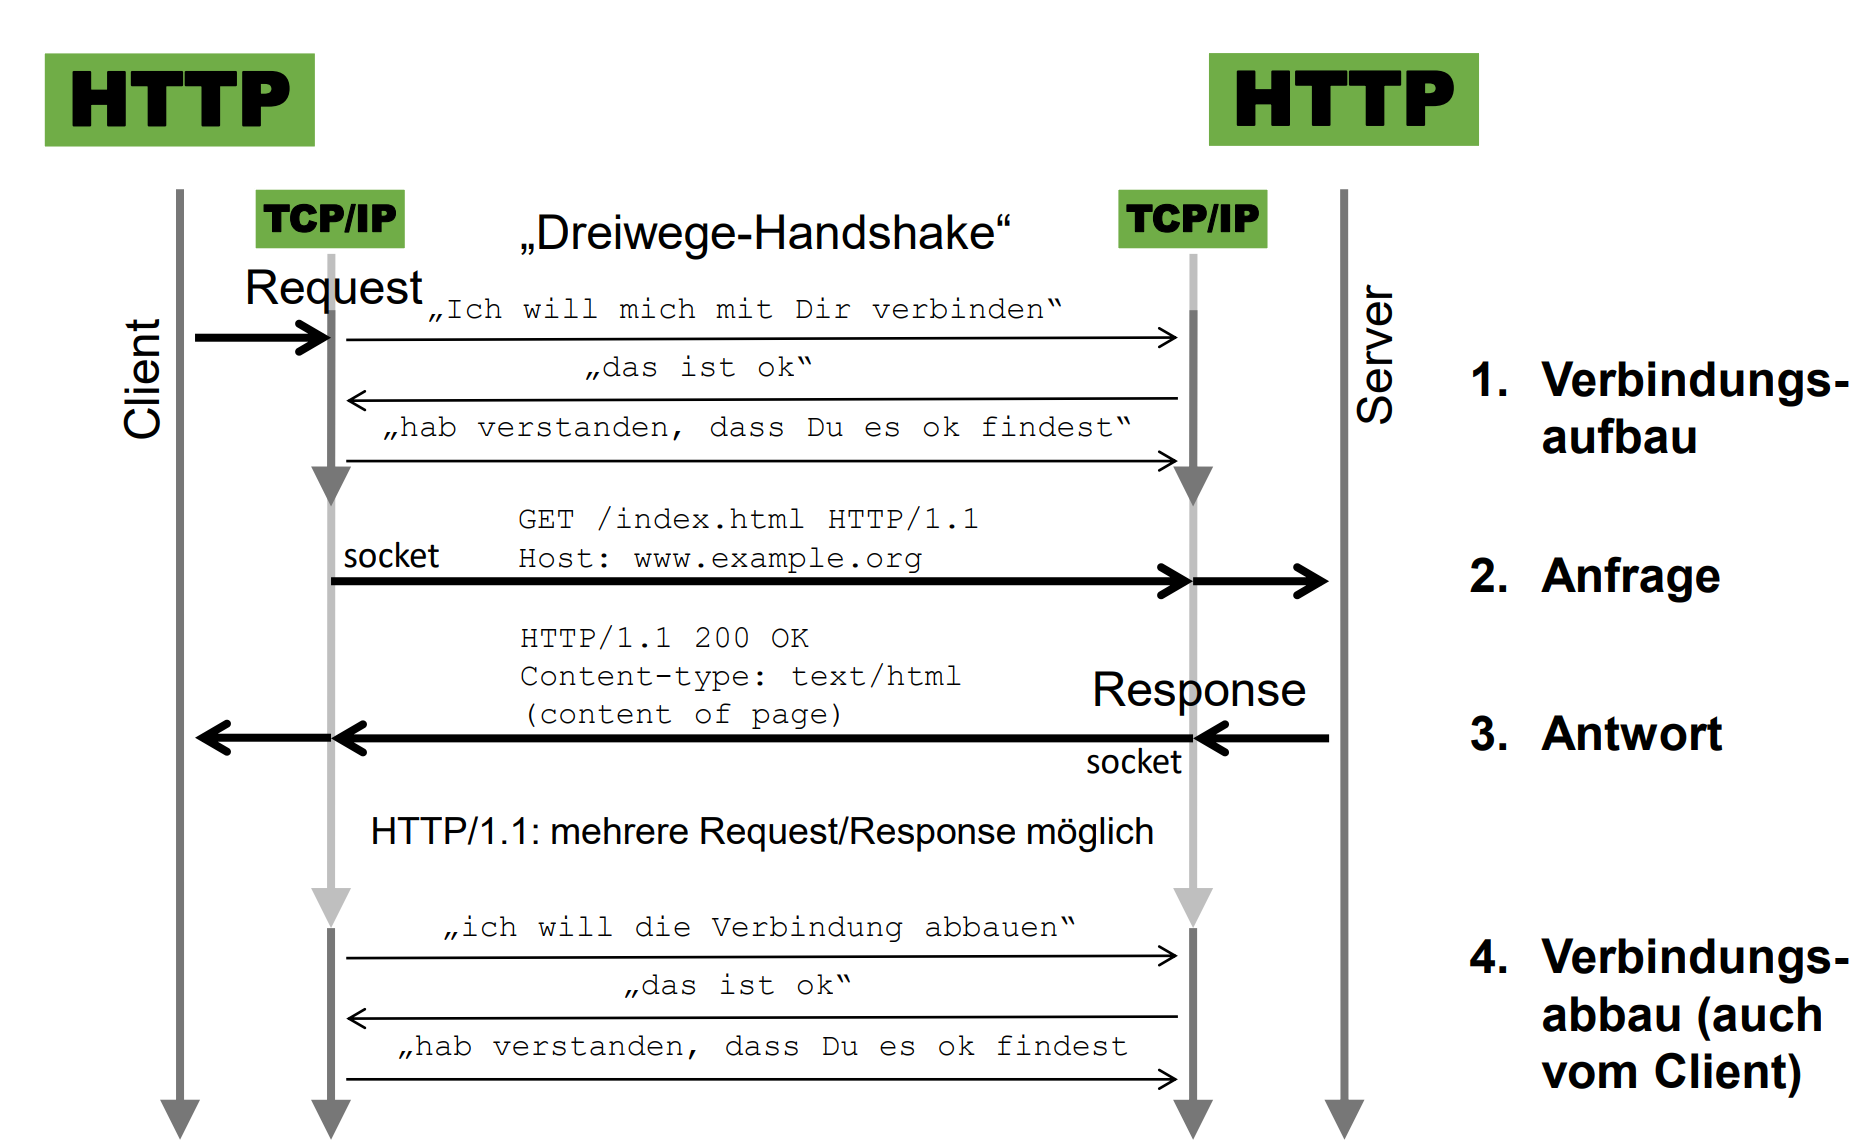
\includegraphics[width=\linewidth]{images/handshake}
	\caption{3-Wege-Handshake bei einem HTTP-Request~\cite{Kneisel.2017}}
	\label{fig:handshake}
\end{figure*}

Im Regelfall schickt ein Client zuallererst eine Anfrage an den Server, um herauszufinden, ob dieser überhaupt bereit ist. 
Ist dies der Fall, antwortet der Server mit einer Erfolgs-Antwort, und der Client kann die benötigte Anfrage stellen. 
Wenn der Server die Bearbeitung fertig gestellt hat, sendet er eine Antwort an den Client, der diese zum Beispiel weiterverarbeiten kann (siehe Figure~\ref{fig:handshake}). 
An dieser Stelle ein Alltagsbeispiel, das wohl jeder Internetnutzer kennt: Eine Google-Suchanfrage. 
Navigiert ein Benutzer beispielsweise auf www.google.de, um eine Google-Suche durchzuführen, wird auf dem Gerät des Nutzers (dem Client) zuerst die Webseite mit der Suchleiste von Google geöffnet. 
Gibt der Nutzer nun "Wie wird das Wetter heute" in die Suchleiste ein und betätigt die Suchen-Schaltfläche, wird eine HTTP-Anfrage an den Server von Google gesendet. 
Ist dieser erreichbar und bereit (was wohl die meiste Zeit der Fall sein dürfte), wird der Such-Term in der HTTP-Anfrage versendet. 
Der Server verwendet nun die Rechenleistung eines Rechenzentrums, um die benötigten Antwortdaten zu "berechnen". 
Dafür benötigt er Metadaten wie beispielsweise den Standort des Clients, der ebenfalls in der HTTP-Anfrage mitgesendet werden kann. Nachdem der Server die Wetterdaten für den jeweiligen Standort abgerufen hat, sendet er eine Antwort, ebenfalls mittels HTTP-Protokoll. Der Client, der auf diese Antwort gewartet hat, kann die Informationen nun graphisch aufbereiten und auf dem Display des Nutzers darstellen.
% Statistik: Anzahl Requests/Responses am Tag bzw. Datenmenge
% Überleitung
Dieses Konzept ist zwar in den Jahren entsprechend der Gerätezahl und der HTTP-Kommunikation mit skaliert, stößt jedoch in einigen Punkten an seine Grenzen. An manchen Stellen birgt es sogar große Probleme. Und wenn man sich mit der Kritik am Web~2.0 befasst, sind technische Gegebenheiten nicht immer das Problem, in vielen Fällen aber die Ursache, weshalb die Rufe nach Dezentralisierung lauter werden.
% Beleg
Aufgrund dessen spielt das Verständnis der dem Internet zugrunde liegenden Technik mindestens aus konzeptioneller Sicht eine nicht unerhebliche Rolle.


%\subsection{Aktuelle Situation}
% ca. 0,5 Seiten

% Entwicklung seit der Dotcom-Blase (was macht die Phase Web~2.0 aus):
%	- bunteres Web
%	- Partizipation von Nutzern
% TBLee: Mag Begriff Web~2.0 nicht
% Plattformen als "Mittelsmänner", denen Vertraut werden muss (+ Beispiele)


\subsection{Kritik und Problematik}
% ca. 3 Seiten

Doch nun zu den Gründen, warum es überhaupt Menschen gibt, die sich mit dem Einsatz von neuen Techniken in der nächsten Generation des Internets beschäftigen. Wie bereits erwähnt hat sich das Internet schnell sehr stark entwickelt, um nicht zu sagen verändert. Dennoch basiert das grundlegende technische Konzept auf den Anfang der neunziger Jahre erfundenen Webservern. Doch wieso ist das schlecht, es funktioniert doch alles, oder? 
Diese Aussage ist theoretisch richtig, doch durch diese Struktur entstehen Probleme, die nicht auf den ersten Blick sichtbar sind und die viel zu lange inkonsequent behandelt wurden. Um das gewichtigste Problem an den Anfang zu stellen: Die Kontrolle über die eigenen Daten. Durch die im vorhergehenden Kapitel beschriebenen Plattformen, die als "Mittelsmann" dienen, ist es den Nutzern nahezu unmöglich, Einfluss auf die Speicherung und Verarbeitung der eigenen Daten zu nehmen. Die einzige Möglichkeit ist in den meisten Fällen, auf die Nutzung dieser Dienste oder sogar des gesamten Internets zu verzichten, was in der heutigen Zeit kaum möglich und auch nicht im Sinne des Erfinders ist.
% Kampf von Berners-Lee für freies Internet irgendwo erwähnen
Zudem hat sich die Nutzung von Internet-Plattformen herauskristallisiert, hinter denen riesige Tech-Konzerne stehen, die international agieren und sich geschickt in der Umgehung von lokalen Gesetzen und Auflagen anstellen. Informationen über die Datenverarbeitung sind oft intransparent in seitenlangen Impressen versteckt, sodass diese einfach überlesen werden. Und selbst wenn man sich die Mühe des Entschlüsselns macht, hat man in der Regel keine Wahl: Man vertraut der Plattform mit der Nutzung die eigenen Daten an, oder eben nicht.
% Beispiele für Tech-Giganten und Datenschutzbedenken

Das Unternehmen muss dabei nicht einmal selbst die Daten verkaufen, vermutlich ist dies ziemlich selten der Fall. Dennoch gibt es Andere, die das tun: Meldungen zu Datenschutzskandale in Form von geleakten oder gehackten Daten häufen sich. Zum Teil kursieren Datensätze mit Millionen von Nutzerdaten frei verkäuflich im Internet!
% Belege!

Dies kann nur geschehen, wenn die Systeme der Anbieter nicht ausreichend geschützt sind. Doch Hacker werden immer kreativer, und vor allem für kleinere Plattformen ist es schwierig, die Schutzmechanismen auf dem neuesten Stand zu halten. 
Ein Grund für den Erfolg solcher Datendiebstähle ist, dass die Server in der beschriebenen CS-Struktur sogenannte SPOF's darstellen. Dies steht für \textit{Single Point of Failure} und beschreibt in einem Hardware-System eine Komponente, ohne die das gesamte System nicht Betriebsbereit ist. Das Internet fällt zwar nicht aus, weil eine einzige Webseite offline ist, dennoch kann der Ausfall von verschiedenen Diensten und Plattform verheerende Folgen haben. Diese Ausfälle können sowohl durch Cyber- (oder sogar physischen) Angriffen als auch technischen Defekten entstehen. Diese können in beiden Fällen aufwendig zu Beheben sein und dadurch stundenlange Ausfälle verursachen. Bei Social-Media-Plattformen mag das keine verheerenden Auswirkungen haben, doch es gibt mittlerweile viele kritische Systeme, die ans Internet angeschlossen sind, und von denen zum Teil Leben abhängen.
% Beispiele

\smallskip

\textsc{Recap} Abschließend die größten Probleme des Web~2.0 und damit die Gründe für ein dezentrales Internet zusammengefasst:
\begin{itemize}
	\item Server stellen SPOF's dar, Ausfälle oder Attacken können verheerende Folgen haben
	\item Cyber-Attacken können in Datendiebstählen resultieren, Datensätze werden im Darknet an den meistbietenden verkauft
	\item Der gewöhnliche Verbraucher hat keine Einsicht in die eigenen Daten, geschweige denn die Kontrolle darüber
\end{itemize}

% Stateless einfügen!

\smallskip






\section{Das Web3}

Dieses Kapitel beschäftigt sich nun mit Lösungsansätzen, die die zuvor genannten Probleme mit einer differenzierten Architektur lösen können. Dazu werden einige Beispiele für die Weiterentwicklung des Web~2.0 analysiert und das Web3 am Ende bewertet. Zuvor werden jedoch alle Leser und Leserinnen auf den gleichen Wissensstand gebracht, um den folgenden Ausführungen folgen zu können.

\subsection{Grundlagen und Begrifflichkeiten}

\subsubsection{Dezentralisierung}

Möchte man nun die zuvor analysierten Probleme des Web~1.0 beziehungsweise Web~2.0 umgehen, muss das Internet von der jetzigen Client-Server-Architektur zu einem dezentralen Aufbau wechseln. Das Ausmaß entspricht ungefähr dem von der Entwicklung des Web~1.0 zum Web~2.0. Während man jedoch bei dieser Entwicklung von einer Frontend-Revolution spricht, wird die Umstellung zum dezentralen Web eine Backend-Revolution werden. Der Unterschied? Wie in Kapitel 3 erläutert, charakterisiert das Web~2.0 unter anderem intuitive und nutzerfreundliche Webseiten bis hin zu Webapps. Da diese Seiten für die Nutzer sichtbar sind und sich im Vergleich zu den im Zeitalter des Web~1.0 vorhandenen puren HTML-Seiten radikal weiterentwickelt haben, spricht man von einer Frontend-Revolution. Die Art der Webseiten und -apps in einem dezentralen Internet werden sich jedoch zunächst einmal nicht maßgeblich verändern, sondern nur die zugrunde liegende Technik. Daher ist diese Entwicklung im Backend-Bereich angesiedelt und für den Anwender nicht direkt sichtbar.

Doch wie funktioniert die Dezentralisierung nun eigentlich? Im vorherigen Kapitel über das Web~2.0 wurde erläutert, dass Client-Server-Architekturen einen SPOF darstellen. In Abbildung~\ref{centralized_dezentralized} wird dieser SPOF als \textit{Unique Point of Failure} dargestellt, dem die selbe Bedeutung zukommt. Aus der Abbildung wird der größte Unterschied sehr schnell ersichtlich: In einem dezentralen Netz gibt es keinen Server, auf den alle Clients zugreifen. Stattdessen kann jeder Computer Client und Server gleichzeitig sein. Fällt in diesem Szenario ein Gerät im Netzwerk aus, können die anderen Clients noch immer auf viele andere Computer im Netz zugreifen und so alle Dienste wie gewohnt weiterverwenden.

\begin{figure}
	\centering
	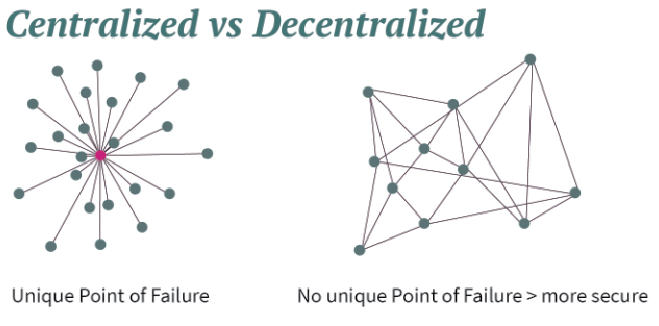
\includegraphics[width=\linewidth]{images/centralized_decentralized}
	\caption{Unterschied zwischen zentraler und dezentraler Architektur~\cite{Blockchainhub.net.2019}}.
	\label{centralized_dezentralized}
\end{figure}


\subsubsection{P2P-Netzwerk}

P2P steht für Peer-to-Peer und bildet im Netzwerk-Kontext das grundlegende Konzept der Dezentralisierung. In einem Peer-to-Peer-Netzwerk sind alle Teilnehmer untereinander gleichberechtigt, wobei jeder Rechner Funktionen, Ressourcen oder Services anbieten oder in Anspruch nehmen kann. Ein \textit{Peer} kann dabei ein einzelner Rechner oder eine Gruppe von Rechnern sein. Ein P2P-Netz kommt ohne Server aus und ist demnach das Gegenteil einer Client-Server-Architektur~\cite{Luber.2018}. 


\subsubsection{Die Blockchain}

Eine wichtige Technologie hin zum dezentralen Web ist Blockchain. Durch die von Satoshi Nakamoto
\footnote{
	Unter diesem Pseudonym wurde im Jahr 2008 das White Paper \textit{Bitcoin: A Peer-to-Peer Electronic Cash System} veröffentlicht, bislang ist unklar ob es sich um eine einzelne Person oder ein Kollektiv von Personen handelt~\cite{BTCAcademy.2018}
}
erfundene Kryptowährung wurde erstmals die Funktion der Währung und damit einhergehend auch der Blockchain erläutert.
Die Blockchain selbst ist eine auf alle Netzwerkgeräte verteilte Datenbank, die sogenannte Blöcke mit Transaktionen enthält~\cite[S. 8]{Crosby.2016}. Diese Transaktionen entstehen zwischen zwei Vertragspartnern und können von jedem Netzwerkteilnehmer verifiziert werden. Für diese Verifizierung wird Rechenleistung benötigt, die von sogenannten Minern für eine bestimmte Vergütung zur Verfügung gestellt wird. Nach der Verifizierung wird die Transaktion in einen Block der Blockchain geschrieben und im Netzwerk distribuiert. Eine Änderung ist ab diesem Punkt nicht mehr möglich, was diese Technik sicher vor Manipulationen und der Abhängigkeit von Vermittlungsplattformen (Intermediären) macht. Wird ein neuer Block hinzugefügt, verweist dieser auf den Hash-Wert des vorherigen Blocks, daher kommt auch der Name \textbf{Blockchain} (zu deutsch: Kette aus Blöcken).

Wie kann jedoch die Sicherheit der Transaktionen garantiert werden? Nun, der Quellcode der Blockchain ist Open Source und daher von allen Nutzern einsehbar. Und darin ist festgelegt, wie mit der Manipulation von einzelnen Transaktionen verfahren wird. Da die verifizierten Blöcke allen Netzwerkgeräten zur Verfügung gestellt werden und somit die "korrekte" Blockchain bekannt ist, werden Änderungen an dieser sofort erkannt und die entsprechenden Geräte aus dem Netzwerk ausgeschlossen. Für eine erfolgreiche Manipulation müssten demnach alle Blockchains auf allen Geräten verändert werden, was schier unmöglich ist.


\subsubsection{Wallet}

Um nun an einem Blockchain-Netzwerk teilhaben zu können, benötigt man ein sogenanntes Wallet. Dies ist eine Software, die bestimmte Algorithmen enthält und auf dem eigenen Client-Gerät ausgeführt wird. 
Um nun an den Vorgängen im Netzwerk teilhaben zu können, werden 2 Keys benötigt: Der Private und der Public Key. 
Der im ersten Schritt generierte Private Key ist ein zufällig-generierter 256-bit Integer, und sollte nicht weitergegeben werden. Er dient dazu, eigene Transaktionen zu signieren. Aus dem Private Key wird im zweiten Schritt mittels \textit{Elliptic-Curve- Cryptography} der Public Key generiert. Diese mathematische Funktion ermöglicht zu jeder Zeit die Ableitung des Public Keys vom Private Key, der umgekehrte Weg (also die Erstellung des Private Keys mittels des Public Keys) würde die leistungsfähigsten Supercomputer mehrere Billionen Jahre beschäftigen. Der generierte Public Key steht auch anderen Nutzern zur Verfügung, und über diesen können Miner verifizieren, ob eine Transaktion tatsächlich von dem Wallet signiert wurde, von dem es vorgibt~\cite[S. 41]{Voshmgir.2019}. 
Aus dem Public Key wird zusätzlich mit einem differenzierten Algorithmus eine Blockchain-Adresse mit Meta-Informationen generiert. Der Algorithmus dient als zweite Sicherungsschicht, für den Fall dass der erste Algorithmus irgendwann mittels Quantencomputern geknackt werden kann. Die Blockchain-Adresse wird wie eine Bankkontonummer verwendet und dient zur eindeutigen Identifikation des Wallet~\cite[S. 42]{Voshmgir.2019}.
Entgegen dem allgemeinen Glauben werden jedoch keine Tokens im Wallet gespeichert. Im Beispiel von Bitcoin heißt dass, das im Wallet keine Bitcoins selbst gespeichert sind. An dieser Stelle ist der Begriff Wallet nicht sehr treffend gewählt, denn darin werden nach dem Private- und Public-Key-Pair alle Transaktionen gespeichert, in denen der Public Key verwendet wurde.
% Beleg (Voshmgir)

Um den Prozess noch einmal abzubilden: Das Wallet (eine Software) enthält Private und Public Key, die Blockchain-Adresse und einige weitere Informationen für spezielle Transaktionen. Zusätzlich werden Einträge gespeichert, die Transaktionen mit dem eigenen Public Key enthalten~\cite[S. 42]{Voshmgir.2019}.
Wird nun eine Transaktion ausgeführt, wird diese auf dem eigenen Gerät mit dem Private Key signiert. Diese signierte Transaktion nennt man \textit{Digital Signature}. Ein anderer Netzwerkteilnehmer kann nun mit der Transaktion und dem Public Key des Senders verifizieren, dass es sich wirklich um denjenigen handelt, der er vorgibt zu sein. Erst nach erfolgreicher Identifikation und Verifizierung wird die Transaktion in die Blockchain geschrieben und an alle anderen Teilnehmer im Netzwerk verteilt. Die Transaktion kann nun nicht mehr verändert werden.

\subsubsection{Smart Contracts}


Smart Contracts sind einem normalen Vertrag ziemlich ähnlich: Zwischen zwei oder mehreren Vertragspartnern geschlossene Vereinbarungen werden darin festgehalten. Dies geschieht jedoch nicht auf Papier, sondern in Form von Programmcode, der in der Blockchain ausgeführt wird. Genau wie die Blockchain selbst ist auch ein Smart Contract Open Source, und auch er kann nachträglich nicht mehr geändert werden. Verträge können somit nicht mehr so leicht verletzt werden. Ein weiterer großer Vorteil ist, dass bestimmte Aktionen automatisch ausgeführt werden können, ohne manuelles Eingreifen zu benötigen. 
Als Beispiel werden oft Lieferketten angeführt: Über die automatische Sendungsverfolgung kann zum Beispiel der Kaufbetrag automatisch überwiesen werden, wenn die Ware beim Kunden ankommt. 
Des weiteren fallen bei Smart Contracts zusätzliche Kosten weg, wie beispielsweise die eines Notars. 
Durch die Dezentralisierung der Verträge ist sichergestellt, dass dieser auch eingehalten wird, und handelsübliche, rechtskräftige Verträge werden nicht mehr benötigt.

Die bekannteste Plattform für die Nutzung von Smart Contracts ist die Plattform \textit{Ethereum}. Diese ermöglicht die Nutzung und Erstellung sogenannter \textit{Dapps}, was für \textit{Distributed Apps} steht (zu deutsch: dezentrale Anwendungen). Durch diese Anwendungen können Smart Contracts erstellt und auf der Blockchain ausgeführt werden~\cite{Ethereum.2019b}. Zudem entstehen zunehmend Anwendungen, die die einfache Erstellung solcher Smart Contracts über eine Oberfläche ermöglichen, sodass auch nicht-Programmierer die Möglichkeit haben, an diesen teilzuhaben.




\subsection{Konzept der Dezentralisierung im Web3}

Doch wie findet nun die Technologie der Blockchain Einsatz in der nächsten Generation des Webs? Da die Blockchain maßgeblich im Zuge der Erfindung der Kryptowährung Bitcoin bekannt geworden ist und diese kontrovers diskutiert wird~\cite{Crosby.2016}, werfen viele die zugrunde liegende Blockchain-Technologie oft mit der Währung in einen Topf. In Wirklichkeit dient sie jedoch für Bitcoin (und andere Kryptowährungen) nur als Mittel zum Zweck, und funktioniert seit deren Einsatz einwandfrei~\cite{Crosby.2016}.
Nichtsdestotrotz denken viele Menschen bei dem Term Blockchain sofort an eine Kryptowährung. Dadurch fällt es schwer, sich auch andere Einsatzgebiete für die Technologie vorzustellen, beziehungsweise wie dieses Konzept aussehen soll. Dazu muss man nun das zuvor erläuterte Konzept der Dezentralisierung mit der Technik der Blockchain in Verbindung bringen: Computer oder Smartphones, wie sie heute bereits in Massen existieren, bilden auf der untersten Ebene die Netzwerkgeräte, die untereinander verknüpft sind. Mit einem darauf aufbauenden Blockchain-Netzwerk können nun verschiedenste Aufgaben erledigt und Dienste angeboten werden, die in Form von den beschriebenen Transaktionen ablaufen. Wichtig dabei ist, dass diese Blockchain-Netze grundlegend auf Tokens aufbauen. Im Beispiel von Bitcoin oder Ethereum sind die Tokens die Währung, in der gehandelt wird. 
Das Bitcoin-Netzwerk nutzt eine gleichnamige Währung (Bitcoin, abgekürzt BTC), im Fall von Ethereum ist die Währung Ether (oder ETH). Tokens sind jedoch ein allgemeines Konzept und unterscheiden sich von Netzwerk zu Netzwerk. 

Tokens sind ebenfalls nicht zwingend eine Währung wie Bitcoin oder Ether, sondern sie können viel mehr Dinge repräsentieren. 
Shermin Voshmgir führt in ihrer Literatur 3 Arten von Tokens an: \textit{Vermögenswerte} (zum Beispiel Strom in Kilowattstunden, Fiat-Währungen
\footnote{
	Fiat-Geld ist eine Währung, die keinen inneren bzw. festen Wert hat, so wie es bei Rohstoffen wie Gold oder Tabak der Fall ist~\cite{CAPinside.2018}. Von Zentralbanken ausgegebenes Geld wie Euro oder Dollar zählen ebenfalls zum Fiat-Geld. 
}, 
Versicherungspolicen oder Event-Tickets), \textit{Zugriffsrechte} (wie Softwarelizenzen, Mitgliedschaften oder Wahlrechte) und eine \textit{Mischform} der beiden (Rechte zum "'minen"' oder native Tokens des jeweiligen Netzwerks (beispielsweise ETH oder BTC)~\cite[S. 151]{Voshmgir.2019}.
Das heißt, dass eben nicht nur mit einer einzigen Währung bezahlt werden kann, sondern viele verschiedene Transaktionen ausgeführt werden können. Manche sprechen sogar von Beispielen, in denen ganze Autos oder Immobilien auf die Blockchain gehoben werden. Dadurch kann beispielsweise ein Testament als Smart Contract aufgelegt werden. Im Todesfall der betreffenden Person wird so das Vermögen auf die Erben verteilt, exakt so wie es im Smart Contract festgehalten ist~\cite[02:10]{Krypto.2018}. 

\smallskip

So wichtig die Blockchain jedoch für das Web3 ist, kann sie allerdings mitnichten als Synonym für den Begriff dienen, wie es ab und zu bei Journalisten oder der Allgemeinheit der Fall ist~\cite[S. 27]{Voshmgir.2019}. Vielmehr ist Blockchain bloß eine Technologie von vielen, die in einem dezentralen Internet Einsatz finden.
Um jedoch den Weg dorthin weitestgehend zu vervollständigen, werden einige andere Protokolle und Techniken benötigt, um die heutigen Dienste mehr oder weniger abbilden zu können. Die Blockchain stellt in diesem Szenario einen großen Nutzen da, um in einem Peer-to-Peer-Netzwerk feststellen zu können, wer was und wann getan hat. Allerdings ist diese nicht dafür geeignet, große Datenmengen zu speichern und zu verarbeiten. Dies hat hauptsächlich 2 Gründe: Erstens sind Blockchains zu langsam und zu rechenintensiv, zweitens bietet die Blockchain nicht immer die richtigen Privatsphäre- und Datenschutzeinstellungen~\cite[S. 27]{Voshmgir.2019}. Zur Größeneinordnung: Die Blockchain des Bitcoin-Netzwerks stieg bis zum dritten Quartal im Jahr 2019 rasant auf eine Größe von knapp 250 GB~\cite{Blockchain.2019}. 

\smallskip

Um nun das Web3 alltagstauglich einsetzen zu können, müssen wenigstens die folgenden Bereiche durch dezentrale Anwendungen abgedeckt werden~\cite[S. 27]{Voshmgir.2019}:

\begin{itemize}
	\item Computerberechnungen
	\item Speicherplatz
	\item Kommunikation und Nachrichtenübermittlung
	\item Monetarisierung
	\item Zahlungsabwicklung
\end{itemize}

Die Blockchain-Technologie kann in diesem Konstrukt mit einem Prozessor in einem Rechner verglichen werden. Er ist für die grundlegende Funktionalität essentiell, benötigt jedoch noch andere Komponenten, ohne die das System nicht anwendbar wäre. 

Mittlerweile gibt es bereits viele dezentrale Anwendungen, die als Lösungen für die oben genannten Komponenten dienen können~\cite{gdamdam.2019}. Viele Protokolle und Plattformen sind noch in der Entwicklung, diese werden jedoch von Zeit zu Zeit besser, indem vor allem zunehmend Unternehmen in diesem Bereich forschen und Entwickeln. Dies belegt vor allem die steigende Zahl der weltweit gegründeten Unternehmen und Start-Ups in dieser Sparte seit 2013~\cite{IPlyticsGmbH.2019}. 

Einige dieser Projekte werden im nächsten Kapitel vorgestellt. Der Fokus liegt dabei darauf, wie diese dezentralen Anwendungen heutige Dienste und Plattformen abbilden oder sogar durch ein neues Konzept ersetzen können. 


\subsection{Dezentralisierung an Alltagsbeispielen erklärt}

Die Beispiele sind in verschiedene Kategorien unterteilt, die allesamt dezentralisiert sind und teilweise sogar aufeinander aufbauen, um eine umfassende Web3-Umgebung zu konzipieren.


\subsubsection{Protokolle und Technologien}

Protokolle und Technologien im Web3 basieren zum Teil auf Blockchain und sollen dabei helfen, verschiedenste dezentrale Anwendungen zu entwerfen und in den Web3-Stack zu implementieren. 


\paragraph{IPFS | InterPlanetary File System}

\begin{figure}
	\centering
	
\includegraphics[scale=0.5]{images/ipfs_logo}
	\caption{Logo des IPFS-Protokolls~\cite{ProtocolLabs.2019}}
	\label{fig:ipfs}
\end{figure}

Das IPFS ist ein Peer-to-Peer-Dateisystem, das den Anspruch erhebt, das HTTP-Protokoll abzulösen~\cite{IdeasEngineering.2018}. In diesem Netzwerk werden Dateien über einen kryptographischen Hash eindeutig identifiziert und auf Netzwerk-Nodes (also einzelne Rechner im Netzwerk) verteilt. Das Konzept orientiert sich dabei an dem Protokoll BitTorrent, das ebenfalls auf den serverlosen Dateiaustausch zwischen Peers setzt. Die Dateien selbst werden jedoch auf jedem der Peers (oder Nodes) in einem Git Repository verwaltet und unterstützen Versionierung~\cite{IdeasEngineering.2018}. Und auch wenn BitTorrent und weitere Protokolle der gleichen Kategorie wie Napster oder KaZaA sehr große Durchsatzraten besitzen, so sind sie dennoch nicht als Infrastruktur ausgelegt~\cite{Benet.2014}.

An diesem Punkt setzt IPFS an, das zwar genau wie HTTP auf TCP/IP aufsetzt, jedoch nicht alleine von diesem Netzwerk-Protokoll abhängig ist. Der größte Vorteil gegenüber HTTP liegt dabei in der Verteilung von vor allem großen Dateien. Diese können sogar in Teilen von verschiedenen Nodes abgerufen werden und sind somit nicht von einer einzigen Bandbreite abhängig. Dieses bietet auch im Streaming enorme Vorteile, vor allem wenn die Datei stark frequentiert ist. Durch das Abrufen eines Videos beispielsweise wird die Datei zur Wiedergabe auf das eigenen Gerät heruntergeladen. Dadurch wird diese jedoch gleichzeitig auch anderen Netzwerkteilnehmern zur Verfügung gestellt, die eventuell sogar geographisch einen kürzeren Abstand besitzen und die Dateien somit nicht mehr um die ganze Welt geschickt werden müssen. Dies funktioniert, da IPFS Inhalte (also Dateien) über deren Hash-Werte adressiert, und nicht wie HTTP über Speicherorte. Wird eine Website über HTTP(S) über einen Domainnamen aufgerufen, wird dieser Name über ein Domain Name System zu einer IP-Adresse und einem Speicherort auf dem adressierten Server aufgelöst. Bei IPFS hingegen sucht sich das Netz bei einem Dateiaufruf die am nächsten gespeicherte Datei, was einen enormen Geschwindig-keitsvorteil darstellt und zusätzlich Ausfallsicherheit gewährleistet~\cite{CodersBlog.de.2019}
Davon abgesehen ist auch ein Dateizugriff möglich, wenn bestimmte Netzwerk-Bereiche durch beispielsweise Zensur oder Naturkatastrophen abgeschnitten sind~\cite{IdeasEngineering.2018}.

\smallskip

\textsc{Sidenote:}
\textit{
	Nachdem die Zentralregierung in Madrid verschiedene Domains hat sperren lassen, die zur Organisation des katalanischen Referendums zur Unabhängigkeit dienten, veröffentlichte der katalanische Präsident Puigdemont einen Link auf eine Datei in einem IPFS-Netzwerk~\cite{Winters.2017}. Da heutige Browser das IPFS-Protokoll noch nicht implementiert haben, muss der Dateiaufruf über einen Webserver auf HTTP umgeleitet werden~\cite{IdeasEngineering.2018}, die Datei selbst mit Informationen über das Referendum am 01. Oktober 2017 war jedoch in einem dezentralen Netz verfügbar.
}


\paragraph{Blockstack}

Blockstack ist ein dezentrales Internet und bietet eine Plattform für die Entwicklung dezentraler Apps und verschiedensten Öko-Systemen. Die beiden Gründer des New Yorker Unternehmens, Muneeb Ali und Ryan Shea, wollen damit gegen die Macht, Einflussnahme und Vorherrschaft der GAFA-Konzerne
\footnote{
	\textbf{G}oogle, \textbf{A}pple, \textbf{F}acebook und \textbf{A}mazon
}
vorgehen~\cite{Kyriasoglou.2018}. Der Schwerpunkt liegt dabei auf Datensicherheit durch Verschlüsselung und Privatsphäre. Da alle Daten verteilt und nicht auf einem zentralen Server gespeichert sind, hat der Nutzer ständige Kontrolle, inklusive der vollständigen Löschung seiner gesamten Daten~\cite{Kyriasoglou.2018}.


\subsubsection{Databases}


\paragraph{BigchainDB}

\begin{figure}
	\centering
	
\includegraphics[scale=0.5]{images/bigchaindb_logo}
	\caption{Logo-Schriftzug der Bigchain-Datenbank~\cite{Vecta.io.2019}}
	\label{fig:bigchaindb}
\end{figure}

Die vom Berliner Startup \textit{Ascribe} ins Leben gerufene Datenbank BigchainDB setzt ebenfalls auf die Blockchain-Technologie. Sie soll, wie andere dezentrale Anwendungen auch, "'dezentralisierte Kontrolle, Widerstandsf{\"a}higkeit gegen Manipulationen [sowie] Erzeugung und {\"U}bertragung von Werten"'~\cite{Schmiechen.2016} bieten. Dabei deckt sie ein weitläufiges Einsatzgebiet ab, sowohl für Privatpersonen als auch für Unternehmen. Dazu zählen unter anderem~\cite{Schmiechen.2016}:

\begin{itemize}
	\item \textbf{Verbindliche Verträge} mit allen dazugehörigen Transaktionen können direkt in der BigchainDB gespeichert werden.
	\item \textbf{Erzeugung und sofortige Übertragung von großen Vermögen.} Nur der Besitzer der Vermögen kann diese übertragen. Nicht der Netzwerkadministrator, wie in bisherigen Datenbanksystemen. Kosten werden minimiert, alles soll schneller gehen.
	\item \textbf{Echtzeit-Verfolgung der Produktion von Gegenständen.} Zum Beispiel indem Daten von RFID-Chips in Bigchain gespeichert werden. So sollen Kosten gespart und Betrug vermieden werden.
	\item \textbf{Nachhalten von Urheberrechten.} Digitale Kunstwerke oder Musik kann mit einem Wasserzeichen versehen werden. Alle Informationen über die Verbreitung und Kopien werden dann in der Bigchain gespeichert. Der Lizenzinhaber behält den Überblick über die Verbreitung seiner Werke. Auf dieses Feld hat sich Ascribe konzentriert.
	\item \textbf{Zeitstempel, Zertifikate und Quittungen.} Bigchain ist in der Lage, digitale Vorgänge offen zu legen. Wann wurde was übertragen? Das verhindert juristische Probleme bei Vertragsabschlüssen.
	\item \textbf{Verbesserung der Verlässlichkeit von Datenbanken.} Bis jetzt kann ein einziger Fehler zu Datenlecks führen. BigchainDB kann das verhindern.
\end{itemize}

Der größte Vorteil liegt jedoch zweifelsohne in der Geschwindigkeit: Durch den dezentralen Ansatz soll die Datenbank in der Lage sein, mehr als eine Million Vorgänge pro Sekunde abzuarbeiten. Dies ermöglicht die hohe Skalierbarkeit, die zu Anfang des Produkts nicht gegeben war~\cite{Schmiechen.2016}. 


\paragraph{IPDB | InterPlanetary Database}

Nicht zu verwechseln mit der \textit{Internet Pinball Machine Database} (erreichbar unter ipdb.org) verspricht die Webseite unter ipdb.io eine neue Datenbank für das dezentrale Web. Die von \textit{The Interplanetary Databse (IPDB) Foundation e.V.}, einer deutschen Non-Profit-Organisation, ins Leben gerufene Datenbank baut auf der zuvor beschriebenen BigchainDB und dem IPFS auf~\cite{IPDB.2018}. Das Projekt wird derzeit von einem Konsortium von Organisationen unterstützt, die die Idee einer gut verwalteten Blockchain-Datenbank unterstützen~\cite{IPDB.2018}. Shermin Voshmgir sieht diese Datenbank hauptsächlich im Gebiet der Metadaten-Speicherung in einem P2P-Netzwerk~\cite[S. 29]{Voshmgir.2019}. 


\subsubsection{Datenspeicherung und -freigabe}

\paragraph{Storj}

Diese im Jahr 2014 als Open-Source gegründete Plattform ist die dezentrale Dropbox (oder Google Drive). Storj wird in diesem Fall wie "Storage" ausgesprochen~\cite{Blockchainwelt.2019}. Das in Atlanta ansässige Unternehmen Storj Labs bietet sein Produkt im Prinzip als zweiseitige Medaille an. Auf der einen Seite stehen die sogenannten \textit{Farmer}, die eigenen Speicherplatz bereitstellen und dafür entlohnt werden. Wer nun eigene Dateien in der Cloud speichern möchte, mietet sich dafür einfach Speicherplatz. Dieser Speicherplatz wird jedoch nicht auf einem einzigen Geräte bereitgestellt, vielmehr werden die hochgeladenen Dateien in Fragmente, sogenannten \textit{Shards}, unterteilt und auf viele verschieden Farmer verteilt~\cite{Blockchainwelt.2019}. 

\smallskip

\textsc{Sidenote:}
\textit{
	Ein Farmer in einem Storj-Netzwerk kann auch als Node oder Peer bezeichnet werden. 
}

\smallskip

Hauptaugenmerk bei dieser Anwendung liegt auf der Ende-zu-Ende-Verschlüsselung und die Fragmentierung der einzelnen Dateien. Selbst wenn es einem Angreifer gelingen würde, die Verschlüsselung zu knacken, hätte er nur ein Fragment der Datei, und ohne die Speicherorte der anderen Fragmente kann die Datei kaum gelesen werden. Die Information über die Speicherorte der einzelnen Fragmente besitzt jedoch nur der Eigentümer der Datei, was einen Höchstgrad an Sicherheit garantiert~\cite{Blockchainwelt.2019}.


\paragraph{Sia}

Das Konzept des Speicheranbieters Sia ist dem von Storj sehr ähnlich. Hier besitzt ein Nutzer der Cloud sogar einen eigenen privaten Chiffrierschlüssel. Der Zugriff auf die Dateien erfolgt automatisch mittels einem Smart Contract, was zusätzliche Sicherheit gewährt. Zudem gilt auch hier, dass niemand anderem (vor allem einer fremden Person oder einem fremden Unternehmen) vertraut werden muss, und trotzdem sind die Daten redundant und damit ausfallsicher in der Cloud abgelegt~\cite{Sia.2019}.


\paragraph{Swarm} Diese verteilte Speicherplattform setzt auf dem Web3-Stack der Plattform Ethereum auf, und ermöglicht Entwicklern die Nutzung von redundantem Speicher, etwa für Dapp-Code, Benutzerdaten oder Metadaten zur Blockchain~\cite{Swarm.2019}. Swarm ist Teil der Roadmap von Ethereum hin zu einem dezentralen Internet. Es existiert dabei neben Smart Contracts und Whisper als dezentrale Nachrichtenübermittlung und stellt daher einen essentiellen Part dar~\cite{Gerring.2016}.

% Ggf. weitere Beispiel einfügen

\medskip

Abschließend lässt sich festhalten, dass es eine zunehmende Anzahl von dezentralen Netzwerken und Anwendungen gibt, die mehr oder weniger auf Blockchain basieren. In folgendem GitHub-Repository von \textit{gdamdam} (\url{https://github.com/gdamdam/awesome-decentralized-web}) ist eine Liste von dezentralen Technologien zu finden, die noch immer erweitert wird.



\subsection{Vor- und Nachteile}

\textsc{Recap:} Viele Vorteile des dezentralen Webs wurden bereits in den vorhergehenden Ausführungen angesprochen und erläutert, zur Vollständigkeit werden nachfolgend die Wichtigsten erneut aufgelistet:

\begin{itemize}
	\item \textbf{Ausfallsicherheit:} In einem verteilten Netz gibt es keinen Single-Point-of-Failure, was erhöhte Datenverfügbarkeit in den meisten Bereichen mit sich bringt.
	\item \textbf{Schutz vor Angriffen:} Blockchain-basierte Netzwerke und Anwendungen besitzen viel höhere Sicherheitsmaßnahmen, beispielsweise durch starke Verschlüsselungsalgorithmen. Zudem können Angriffe nicht auf einen einzigen Server konzentriert werden, um beispielsweise Daten zu stehlen oder einen Ausfall zu verursachen.
	\item \textbf{Datenschutz und Privatsphäre:} Nutzer sind Eigentümer über die eigenen Daten und müssen diese keinen Intermediären anvertrauen. Sie haben bei korrekter Anwendung (wie zum Beispiel Geheimhaltung des Private Keys) die alleinige Kontrolle über die eigenen Daten, können frei über diese verfügen und sie gegebenenfalls löschen. Auch der Schutz vor Angriffen bewirkt eine enorme Senkung der Eingriffe in die Privatsphäre der Nutzer.
	\item \textbf{Keine Intermediäre:} Dieser Punkt birgt Vorteile in vielen Bereichen. Durch den Wegfall der Vermittlungsplattformen können enorme Kosten und Wege gespart werden, dies zudem bei höchstem Datenschutz.
	\item \textbf{Smart Contracts:} Bereits heute gibt es eine Vielzahl von Anwendungsfällen, die viele Vorgänge einfacher und sicherer gestalten können. Diesen ist nach oben hin keine Grenze gesetzt, und Smart Contracts haben die Möglichkeit, sowohl das Privatleben als auch die Prozesse von Unternehmen massiv zu verändern.
\end{itemize}

\smallskip

Diese Punkte jedoch so stehen zu lassen, wäre nicht korrekt, denn die Entwicklung dieser Protokolle und Anwendungen hat quasi gerade erst begonnen. Durch den Anstieg an Unternehmen, die sich in diesem Bereich angesiedelt haben, stehen mehr und mehr Ressourcen für Forschung und Entwicklung zur Verfügung, dennoch müssen viele Probleme erst noch gelöst, geschweige denn erkannt werden. Und auch wenn es für viele der heutigen Anwendungen bereits dezentrale Lösungen gibt, fehlt es dennoch an einer Auswahl an etablierten Netzen und Plattformen, um einen produktiven Einsatz zu gewährleisten. 

Des Weiteren steht und fällt eine Anwendung mit ihrer Programmierung. Auch wenn Bugs heute bereits fatale Folgen haben können, ist die Entwicklung mit bekannten Techniken in den allermeisten Fällen serienreif, und immer beliebter werdende Test-Frameworks und -Prozesse sichern die korrekte Ausführung der Programme. Da viele dezentrale Projekte den Open-Source Ansatz verwenden, greift in diesen Fällen das Vier-Augen-Prinzip, was die Fehlersuche beschleunigen kann. Dennoch werden dafür auch genügend Entwickler benötigt, die dieser Aufgabe nachkommen und die dafür qualifiziert sind. 

Vor allem bei den Smart Contracts können Programmierfehler ein hohes Risiko bergen. So verlässlich und automatisiert sie in ihrer Ausführung sind, so sicher werden eben auch Probleme bei falscher Programmierung verursacht, wie das folgende Beispiel zeigt.

\smallskip

Dem Wagniskapitalgeber \textit{The DAO}, der im April 2016 mit 150 Millionen US-Dollar aus einer Crowdfunding-Kampagne startete, wurde dies zum Verhängnis. The DAO war eine \textbf{d}ezentrale, \textbf{a}utonome \textbf{O}rganisation (daher der Name), die mithilfe von Smart Contracts in Unternehmen, vor allem in Start-Ups investieren wollte. Der Unterschied zu anderen Venture-Capital-Firmen? Die Organisation kommt ohne Management oder Direktoren aus, stattdessen werden die Entscheidungen für Investitionen automatisch mit Smart Contracts getroffen~\cite{Reiff.2019}.
The DAO setzte auf Ethereum auf und benutzte dessen Währung ETH. Bereits im Juni des selben Jahres gelang es jedoch einem Nutzer, über einen längeren Zeitraum insgesamt Ether im Wert von ungefähr 50 Millionen US-Dollar auf sein eigenes Konto umzuleiten~\cite{Reiff.2019}. Während die Gründer überlegten, wie sie das Geld zurückholen können, bekamen sie einen Brief des "Diebs", und darin drohte dieser The DAO mit rechtlichen Schritten! Er gelangte nämlich durch einen Programmierfehler eines Smart Contracts an die Tokens, und auch wenn sein Verhalten unethisch war, illegal war es nicht~\cite[05:08]{Krypto.2018}. Letztendlich erhielt er das Geld nicht, dennoch führte der "Diebstahl" bereits im September 2016 zum Ende von The DAO~\cite{Reiff.2019}. 

Das Ethereum-Netzwerk wurde einem Hard-Fork unterzogen. Das heißt es gibt derzeit 2 Versionen von Ethereum: Eine alte, in der der Programmierfehler immer noch existiert, und eine neue, wo der Fehler durch Updates der Ethereum Nodes behoben wurde. Und obwohl die Ethereum-Community mehrheitlich für den Hard-Fork gestimmt hatte, spaltete der Vorfall die Nutzerschaft, denn dieser sei nicht im Sinne eines führerlosen und dezentralen Systems~\cite{Hayes.2016}. 






\section{Ausblick}

Nachdem nun die aktuelle Situation des heutigen Internets aufgezeigt und die möglichen Entwicklungen in der Zukunft erläutert wurden, soll das letzte Kapitel sich damit beschäftigen, inwieweit die Dezentralisierung im Bezug auf das Internet Einzug finden kann beziehungsweise wird.

\begin{figure*}
	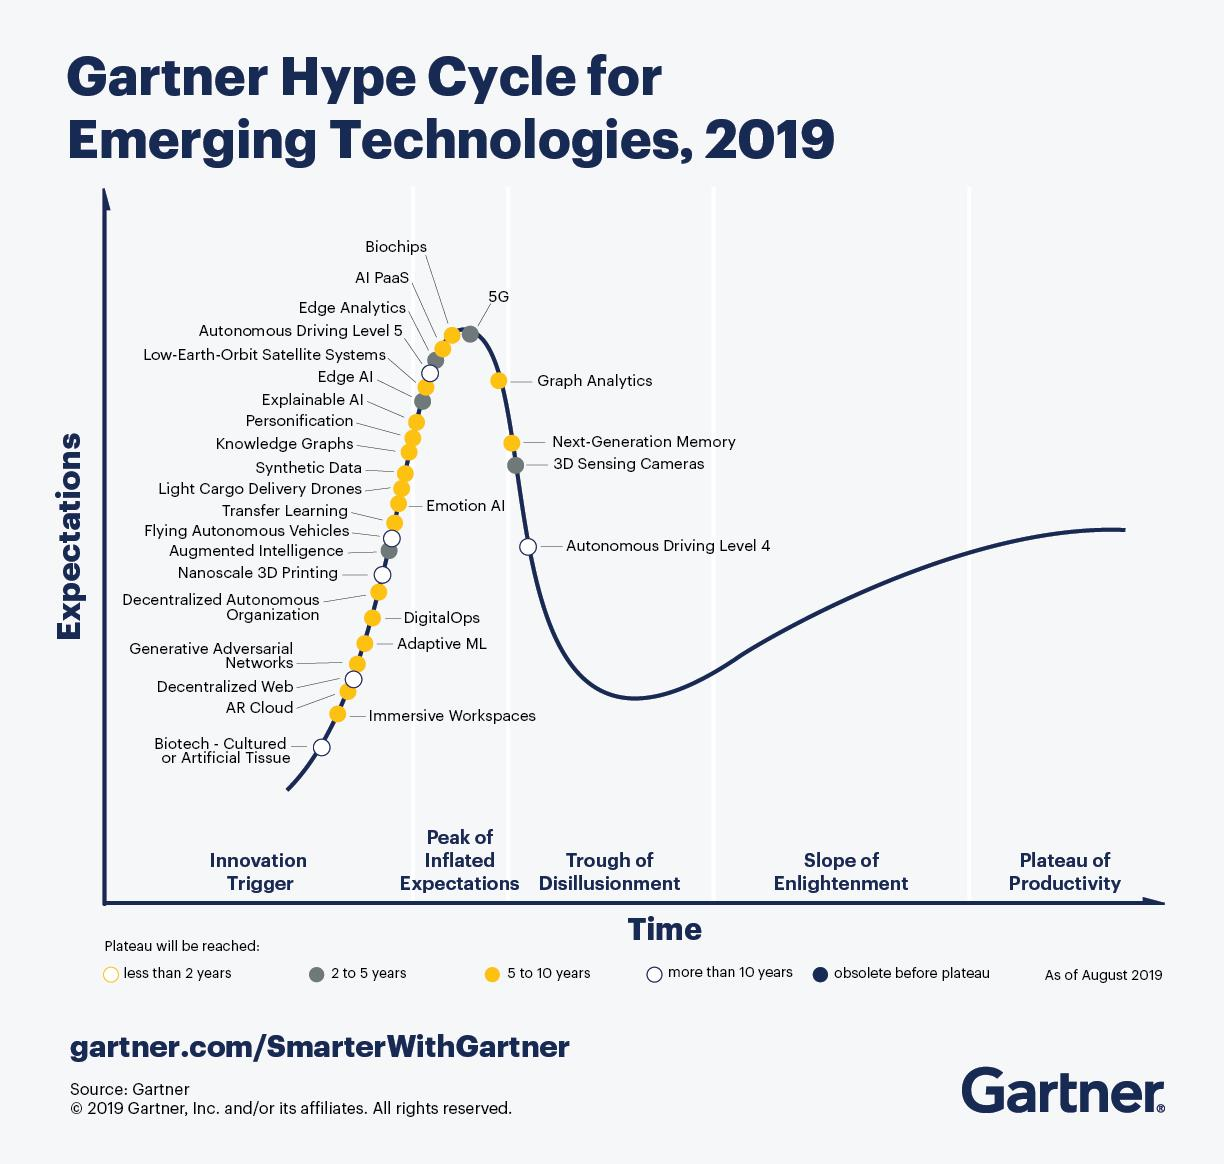
\includegraphics[width=\linewidth]{images/5TrendsAppear.jpg}
	\caption{Gartner Hype Cycle for Emerging Technologies, 2019~\cite{Panetta.2019}}
	\label{fig:gartnerhype}
\end{figure*}

Wie in Figure~\ref{fig:gartnerhype} zu sehen, befindet sich die Technologie \textit{Decentralized Web} noch ziemlich am Anfang des Gartner Hype Cycle's, und der Zeitraum bis zur Etablierung ist auf 10 Jahre geschätzt. 
Wie bereits angesprochen, sieht man immer mehr Unternehmen, Organisationen und damit letztlich Menschen an der Technologie arbeiten. Dies liegt hauptsächlich daran, dass es die heutigen Tech-Konzerne mit der Verletzung der Privatsphäre zu weit getrieben haben. Letztendlich arbeiten viele Personen freiwillig an der Technologie, weil sie für ein freies Internet kämpfen, in dem die Nutzung von Diensten nicht mit seinen privaten Daten "'erkauft"' wird. Denn nichts anderes passiert in der jetzigen Zeit des Web2: Die frühen Anbieter von Services im Internet haben sehr schnell mitbekommen, dass Nutzer nicht bereit dafür sind, für die Nutzung der Dienste im Web zu bezahlen. Also suchten sie nach anderen Möglichkeiten, Profit zu generieren, und dadurch entwickelte sich die heutige Kommerzialisierung mit Nutzerdaten.


Und dieses Konzept war nie im Sinne des Erfinders. Der durch seine Pionier-Arbeit am World Wide Web zum Ritter geschlagene Sir Timothy Berners-Lee hat nie auch nur ansatzweise ein Vermögen mit seiner Erfindung verdient, er wollte lediglich das Leben der Menschen verbessern und vereinfachen. 
Nun arbeitet er schon länger am sogenannten Solid-Projekt~\cite{Clark.2018}. 
Die Abkürzung steht für Social Linked Data und zielt darauf ab, den großen Technik-Firmen die Nutzerdaten aus ihren Daten-Silos zu entziehen und diese in sogenannten Pods zu speichern, die der Nutzer selbst kontrolliert. 
So soll beispielsweise ein Umzug von Firma A zu Firma B problemlos möglich sein: Man entzieht A ganz einfach die Berechtigung auf den eigenen Datenpod und gewährt sie B~\cite{Park.2018}. 

\smallskip

Dies wird jedoch schwieriger, als auf den ersten Blick ersichtlich: Die Konzerne, gegen die das Projekt gerichtet ist, werden sich wohl kaum an einer einheitlichen Lösung beteiligen, und für neue oder kleine Firmen fehlt es an Nutzerzahlen und damit an Investoren~\cite{Park.2018}. Dieses Problem entstand laut Steven Johnson, weil die von ihm als "'InternetOne"' bezeichnete Schicht offene Protokolle wie TCP/IP und HTML verwendeten, und die Verwaltung von Identitäten und persönlichen Daten auf das "'InternetTwo"' ausgelagert wurden. Die Protokolle dieser zweiten Schicht wurden jedoch vornehmlich von Unternehmen definiert, weshalb kaum Standards im Bereich der Datensicherheit existieren~\cite{Bonset.2019}. 

\smallskip

All das Engagement zeigt, dass vor allem das Thema der Privatsphäre und des gläsernen Bürgers in den Vordergrund rückt. Doch eine schnelle Änderung der Situation wird dies wohl nicht bewirken, dafür verzeichnen die etablierten Plattformen zu große Nutzerzahlen, und es gibt noch zu wenige beziehungsweise keine konkurrenzfähigen Alternativen.

Vermutlich werden in der Zukunft Unternehmen die Technologie der Dezentralisierung weiter vorantreiben und auch einsetzen, bevor diese vollumfänglich in den privaten Sektor vordringt. Denn durch die Blockchain stehen vor allem Unternehmen enorm viele Möglichkeiten offen, da diese nicht nur Prozesse vereinfachen und automatisieren kann, sondern auch hohe Kostensenkungen ermöglicht.

Fakt ist, dass die Technologie noch viele Jahre zur Marktreife benötigt. Nichtsdestotrotz stellt sie jedoch eine realistische Alternative zum Marktmonopol einiger weniger Unternehmen dar, und diese Alternative wird mit zunehmenden Jahren immer dringender benötigt. Die Veränderung zum dezentralen Web wird jedoch nach und nach Anklang finden, je nachdem wie die Entwicklung voranschreitet und die Technik in der Gesellschaft angenommen wird.








% Literaturliste endgueltig anzeigen
\bibliography{Quellen}

\end{document}
\endinput